\documentclass{cours}

\title{\textsc{Etude Computationnelle de la Stabilité Interlangue des Catégories Morphosyntaxiques}\\
{\small Rapport de Stage de L3} }
\author{Matthieu Boyer}

\newcommand{\codedir}{Morphosyntactic-Categories_Code}
\usepackage{nicematrix}

\begin{document}

    \begin{abstract}
        Dans ce rapport, nous nous intéressons à la stabilité interlangue des catégories morphosyntaxiques.
        Nous avons quantifié la manière dont différentes catégories descriptives d'un langage ont différentes
        significations dans différents langages,
        et particulièrement la manière dont un concept est matérialisé dans différents langages.
    \end{abstract}


    \section{Pourquoi?}
    Cette citation de Martin Haspelmath sur la différence entre une catégorie linguistique descriptive dans un langage et une catégorie linguistique comparative dans le méta-langage est le point de départ de notre étude.
    \begin{quote}
        There is a fundamental distinction between language-particular categories of languages (which descriptive
        linguists must describe by descriptive categories of their descriptions) and comparative concepts (which
        comparative linguists may use to compare languages).
        {\flushright
    {\textit{Martin Haspelmath} \cite{Has18}}}
    \end{quote}
    Selon Haspelmath, il est possible que la manière de décrire les langues en linguistique soit basée sur des envies de comparaison, parfois mal placées.
    Dans ce rapport, nous allons donc nous intéresser à la notion fondamentale de catégorie morphosyntaxique, et
    comparer les descriptions dans différents langages de catégories linguistiques comparatives.

    \section{Données et \emph{Universal Dependencies}}
    Pour étudier la thèse d'Haspelmath, nous allons considérer que les relations de dépendances (\textit{reldep}) décrites par les annotations de \textsc{Universal Dependencies} (UD, version 2 décrite dans \cite{UDv2}) sont une manière de représenter des catégories comparatives.
    Une relation de dépendance est une manière de décrire les relations syntaxiques dans une phrase.
    Elles se déduisent de la construction par une grammaire de dépendance ou contextuelle de la phrase.
    \begin{figure}[H]
        \centering
        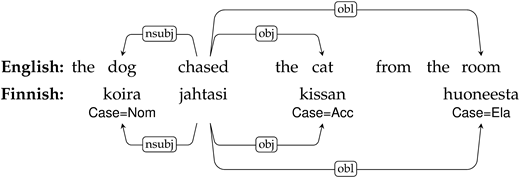
\includegraphics[width=\textwidth]{\codedir/Figures/Visualisations/simplified_ud_annotation.png}
        \caption{Représentation d'une phrase et de ses relations de dépendances en anglais, source:\cite{UDv2}}
    \end{figure}
    Il existe 37 relations de dépendances de base, mais les personnes annotant les corpus ont la possibilité d'en créer de nouvelles, sous la syntaxe \texttt{str1:str2:\dots} où \texttt{str1} doit être une relation de dépendance décrite comme relation basique dans la table 3 de \cite{UDv2}.\\
    Par ailleurs, les mots sont annotés avec les propriétés morphologiques qu'ils possèdent, par exemple leur temps ou leur aspect pour un verbe ou leur cas et leur genre pour un nom.
    Les propriétés morphologiques universelles utilisées par UD sont décrites table 2 dans \cite{UDv2}.\\
    Enfin, les mots sont annotés avec leur nature grammaticale (e.g. Nom, Verbe, Pronom\dots) comme décrits table 1 dans \cite{UDv2}.

    \section{Première Approche}
    Nous considérons tout d'abord que chaque \textit{reldep} décrit une unique catégorie comparative et que plusieurs \textit{reldep} ne peuvent instancier une même catégorie comparative.
    En comptant le nombre d'instances de chaque \textit{reldep} pour un mot vérifiant une propriété grammaticale de la langue (i.e.\ une catégorie descriptive, que l'on représente par une \textit{feature} d'UD, typiquement les cas pour des langues en utilisant), on obtient une représentation vectorielle des catégories descriptives et on peut donc mesurer la proximité de deux catégories descriptives dans deux langues différentes.
    Les corpus utilisés dans cette première partie sont ceux du projet \textsc{Universal Dependencies}, version 2.14 décrite dans \cite{UD214}.

    \section{Avec la distance Cosinus}
    On mesure en utilisant la distance Cosinus entre deux vecteurs la proximité entre ceux ci: \begin{equation}d_{\cos}(v_{1},v_{2}) = \frac{\scalar{v_{1}\mid v_{2}}}{\norm{v_{1}}\norm{v_{2}}}\end{equation}

    On obtient alors les résultats suivants pour quelques cas:

    \renewcommand{\arraystretch}{1.1}
\begin{table}[H]
	\centering
	\resizebox{\textwidth}{!}{\begin{NiceTabular}{ccccccccc}
		Proximity with: & Abl & Acc & Dat & Gen & Ins & Loc & Nom & Voc \\
		First Quartile & 0.037 & 0.020 & 0.022 & 0.032 & 0.056 & 0.027 & 0.026 & 0.000 \\
		Median & 0.198 & 0.123 & 0.134 & 0.317 & 0.249 & 0.188 & 0.104 & 0.006 \\
		Third Quartile & 0.416 & 0.302 & 0.341 & 0.823 & 0.449 & 0.400 & 0.225 & 0.047 \\
		Mean & 0.259 & 0.196 & 0.214 & 0.421 & 0.282 & 0.243 & 0.159 & 0.058 \\
	\CodeAfter
		\begin{tikzpicture}
			\foreach \i in {1,...,6}
				{\draw[draw=vulm] (1|-\i) -- (10|-\i);}
			\draw[draw=vulm] (2|-1)--(2|-6);\end{tikzpicture}
	\end{NiceTabular}}
	\caption{Proximities for Case=Gen}
\end{table}

    \renewcommand{\arraystretch}{1.1}
\begin{table}[H]
	\centering
	\resizebox{\textwidth}{!}{\begin{NiceTabular}{ccccccccc}
		Proximity with: & Abl & Acc & Dat & Gen & Ins & Loc & Nom & Voc \\
		First Quartile & 0.020 & 0.038 & 0.018 & 0.026 & 0.035 & 0.020 & 0.620 & 0.003 \\
		Median & 0.067 & 0.137 & 0.072 & 0.104 & 0.113 & 0.078 & 0.815 & 0.026 \\
		Third Quartile & 0.158 & 0.272 & 0.161 & 0.225 & 0.211 & 0.156 & 0.912 & 0.075 \\
		Mean & 0.115 & 0.188 & 0.119 & 0.159 & 0.153 & 0.115 & 0.739 & 0.072 \\
	\CodeAfter
		\begin{tikzpicture}
			\foreach \i in {1,...,6}
				{\draw[draw=vulm] (1|-\i) -- (10|-\i);}
			\draw[draw=vulm] (2|-1)--(2|-6);\end{tikzpicture}
	\end{NiceTabular}}
	\caption{Proximities for Case=Nom}
\end{table}

    \renewcommand{\arraystretch}{1.1}
\begin{table}[H]
	\centering
	\resizebox{.9\textwidth}{!}{\begin{NiceTabular}{ccccccccc}
		Proximity with: & Abl & Acc & Dat & Gen & Ins & Loc & Nom & Voc \\
		First Quartile & 0.000 & 0.000 & 0.000 & 0.000 & 0.000 & 0.000 & 0.003 & 0.500 \\
		Median & 0.004 & 0.007 & 0.006 & 0.006 & 0.012 & 0.007 & 0.026 & 0.885 \\
		Third Quartile & 0.025 & 0.040 & 0.032 & 0.047 & 0.055 & 0.038 & 0.075 & 0.973 \\
		Mean & 0.035 & 0.042 & 0.036 & 0.058 & 0.053 & 0.042 & 0.072 & 0.681 \\
	\CodeAfter
		\begin{tikzpicture}
			\foreach \i in {1,...,6}
				{\draw[draw=vulm] (1|-\i) -- (10|-\i);}
			\draw[draw=vulm] (2|-1)--(2|-6);\end{tikzpicture}
	\end{NiceTabular}}
	\caption{Proximities for Case=Voc}
\end{table}


    On obtient notamment le fait que le nominatif comme le vocatif ont des directions très particulières, et sont très différents de tous les autres cas. Pour le reste, les résultats sont assez flous, et il semble difficile de tirer

    Toutefois, cette méthode est très limitée. En effet, on ne considère ici que 9 des 45 cas définis dans au moins un corpus. Par ailleurs, les résultats donnés ici sont à pondérer par la présence de nombreux corpus/langages ne possédant pas au moins l'un des cas ci-dessus, ce qui amène à une représentation trop brouillée des informations.


    \section{Avec l'algorithme de \textsc{Zassenhaus}}
    On considère les espaces vectoriels engendrés par la représentation vectorielle du système de cas d'une langue, que l'on appellera \textit{espaces de cas}.
    Ceux-ci sont d'une certaine dimension finie.
    On applique alors sur toute paire de système de cas l'algorithme de Zassenhaus, permettant de générer une base de l'espace somme et de l'espace intersection.
    Toutefois, la grande variance au niveau des coordonnées, et la trop faible dimension (au plus 45, mais souvent de l'odrdre de 5) dans un grand espace (dimension 228), rend l'intersection toujours nulle numériquement.
    Par ailleurs, cet algorithme est très lent à exécuter car il demande de nombreux appels mémoire pour obtenir la matrice de l'espace de cas de chaque paire de cas, et demande de trouver une base de l'espace de colonne, ce qui est non-trivialement la matrice.

    \section{Angle entre Cas et Système de Cas}
    On considère à nouveau la distance cosinus, mais cette fois-ci, non pas entre deux vecteurs, mais entre un vecteur et un espace de cas.
    Ceci est fait en considérant le projeté orthogonal d'un vecteur sur un espace de cas et en mesurant l'angle entre les deux (ou la distance cosinus).
    En observant les données de plus près, on trouve une anomalie: l'angle entre le vocatif du farsi et le système de cas arabe est de l'ordre de $\arccos{10^{-16}}$.
    En regardant de plus près les corpus farsis\footnote{et non pas les dindes.}, on observe que cela découle d'une idiosyncracie dans les annotations.
    En farsi, le lemme (unité morphologique abstraite: \textsl{fais} et \textsl{fait} sont deux graphies du même lemme \textsl{faire}, conjugué à deux personnes différentes)
    % \textit{ای}\footnote{Translit=āī}
    est décrit comme une interjection portant le vocatif et se reliant à un nom au cas absolu par la relation de transmission de cas (c'est à dire de marquer le cas pour un autre mot).
    Ce lemme agit donc en réalité plus comme une apposition.
    Le vocatif n'apparaît que très peu en farsi, et majoritairement dans cette situation.
    Ainsi, il semble que nous ne pouvons pas tirer d'enseignements du farsi vers une autre langue, du moins sur le système de cas.
    Il semble toutefois bon de noter qu'il y a sans doute de nombreuses autres anomalies du style dans les corpus.

    Par ailleurs, il n'est pas rare qu'au sein d'une même langue, deux corpus produisent des résultats assez différents. Ceci peut venir de la variance des phrases considérées, mais plus souvent de la présence ou non des reldeps \texttt{conj, case} et de la manière d'annoter le cas d'une apposition (cf. supra).

    \section{Distance Euclidienne}
    On considère cette fois la distance euclidienne entre tous deux vecteurs, qu'on aura au préalable normalisés pour qu'ils représentent des distributions de probabilité.

    \renewcommand{\arraystretch}{1.1}
\begin{table}[H]
	\centering
	\resizebox{.9\textwidth}{!}{\begin{NiceTabular}{ccccccccc}
		Cas & Abl & Acc & Dat & Gen & Ins & Loc & Nom & Voc \\
		Premier Quartile & 0.605 & 0.315 & 0.552 & 0.521 & 0.535 & 0.595 & 0.569 & 0.842 \\
		Médiane & 0.781 & 0.476 & 0.725 & 0.715 & 0.695 & 0.764 & 0.722 & 0.992 \\
		Troisième Quartile & 1.002 & 0.695 & 0.950 & 0.936 & 0.929 & 0.993 & 0.965 & 1.115 \\
		Moyenne & 0.802 & 0.526 & 0.751 & 0.733 & 0.732 & 0.790 & 0.760 & 0.982 \\
	\CodeAfter
		\begin{tikzpicture}
			\foreach \i in {1,...,6}
				{\draw[draw=vulm] (1|-\i) -- (10|-\i);}
			\draw[draw=vulm] (2|-1)--(2|-6);\end{tikzpicture}
	\end{NiceTabular}}
	\caption{Proximities for Case=Acc}
\end{table}


    On utilise ces données pour déterminer, entre deux corpus (ici le Czech-CLTT et le Russian-GSD), quel cas de l'autre langage est le plus proche d'un cas du premier.
    On obtient qu'ici, le datif russe est plus proche du génitif tchèque que du datif tchèque.
    \begin{table}[H]
	    \centering
    \begin{tabular}{>{\tt}r|cccc}
        \toprule
        &Dat RU & Gen CZ & Gen RU & Dat CZ\\
        \midrule
        Total & 1711 & 2631 & 2070 & 277\\
        obl & 450 & 208 & 219 & 48\\
        iobj & 340 & 0 & 0 & 0\\
        amod & 243 & 736 & 475 & 54\\
        nmod & 300 & 1000 & 980 & 24\\
        conj & 112 & 225 & 84 & 21\\
        case & 0 & 340 & 1 & 87\\
        det & 34 & 80 & 79 & 3\\
        \bottomrule
    \end{tabular}
	\caption{Extraits des Vecteurs de Reldep pour le Russe et le Tchèque}
    \end{table}
    On enlève ensuite \texttt{conj, det} puisque ces reldep démontrent l'accord vers la tête, et donc des doublons dans les données, ceci permet d'éviter de compter comme plusieurs instances d'un même cas un groupe nominal de la forme \emph{Alice, le boulanger, la laitière et Bob}, qui remplit un usage sémantique uniforme dans la phrase.
    On enlève aussi case, qui souvent (notamment visible dans l'exemple ci-dessous), est utilisé pour marquer le cas avec une apposition (sur, sous), et ceci dépend très fortement de la personne qui a annoté le corpus, et de l'usage dans les grammaires du langage.\\
    En considérant le graphe orienté des plus proches voisins, on remarque que celui-ci ne peut pas avoir de $n$-cycle pour $n \geq 3$ et décrit des relations de proximité minimale.
    On obtient alors le graphe suivant pour le tchèque et le russe:
    \begin{figure}[H]
	    \centering
	    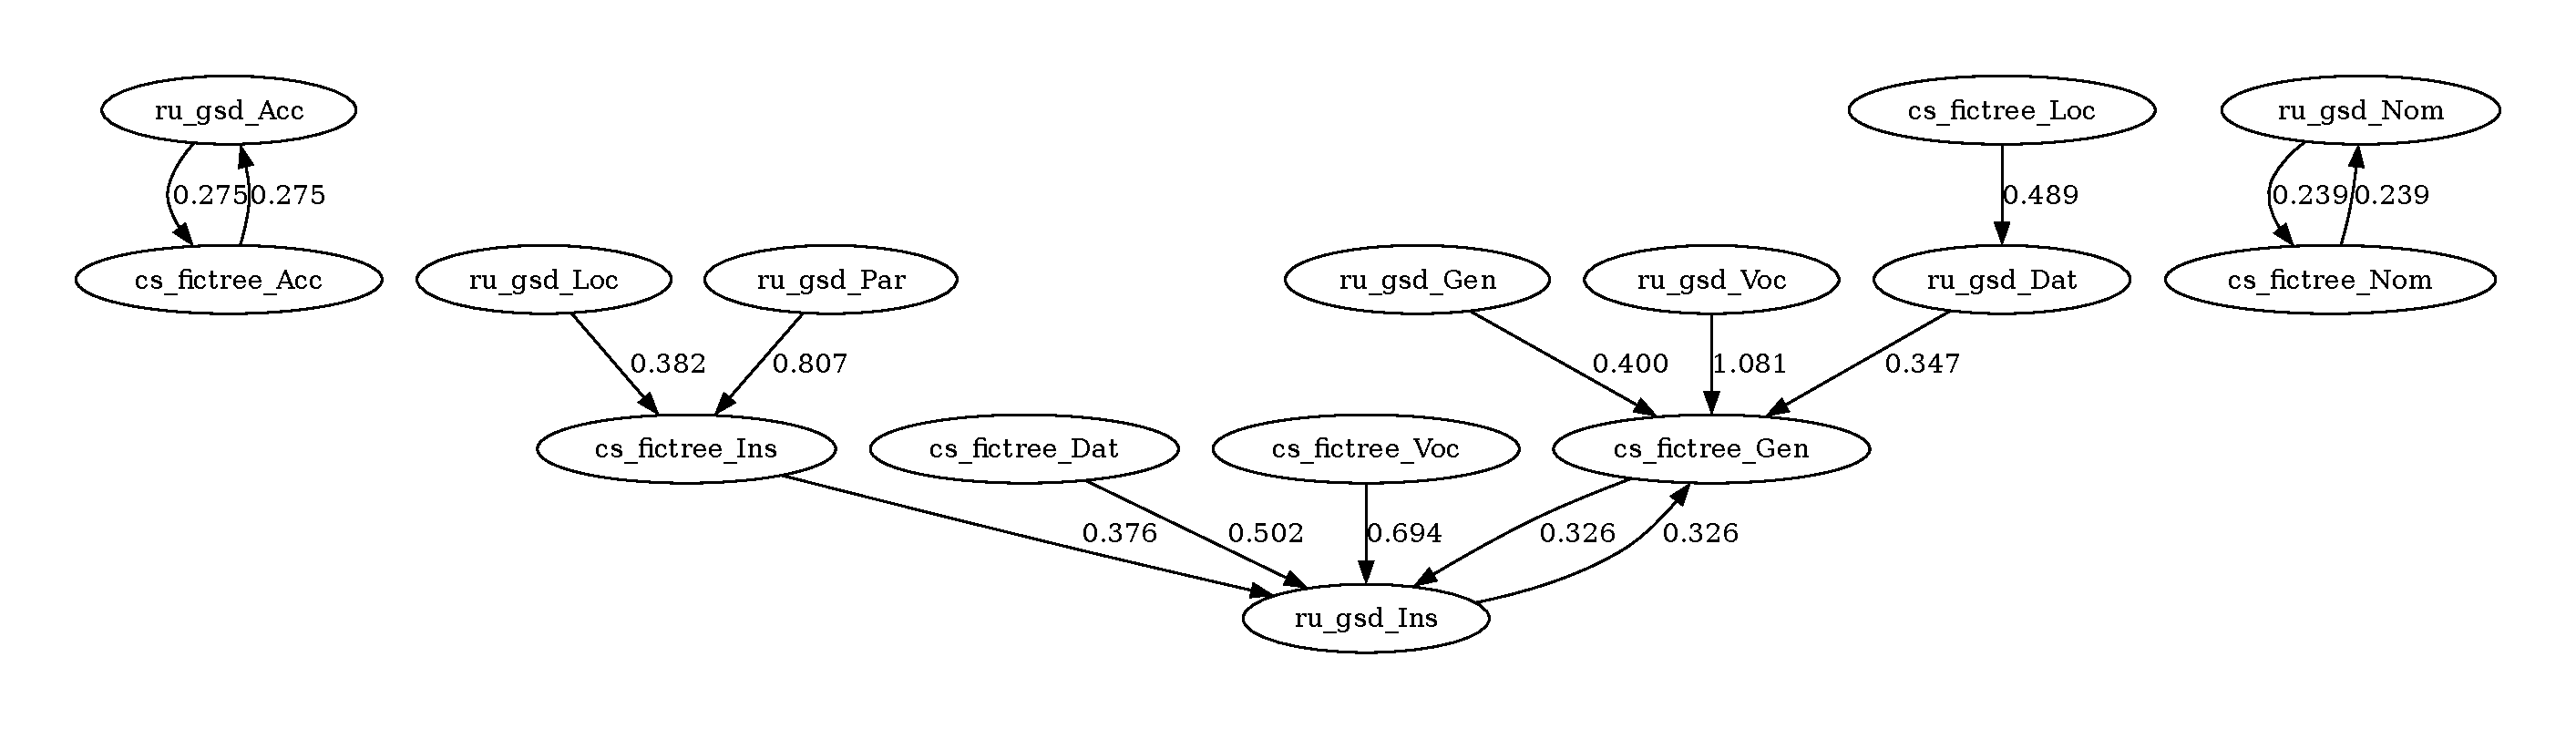
\includegraphics[width=\textwidth]{\codedir/Figures/GNN/gnn_ru_gsd_cs_fictree.pdf}
	    \caption{Graphes des Plus Proches Voisins Russe-Tchèque.}
    \end{figure}
    Pour éviter encore plus d'avoir des redites, on décide de ne se concentrer que sur des mots de même nature.
    Ceci permet par exemple d'éviter qu'un groupe nominal ayant la même fonction sémantique (e.g. objet direct du verbe) apporte plusieurs instances d'un même cas (e.g. avec un adjectif et un nom à l'accusatif).
    On obtient alors le graphe suivant pour le tchèque et le russe en ne considérant que les noms:
    \begin{figure}[H]
	    \centering
	    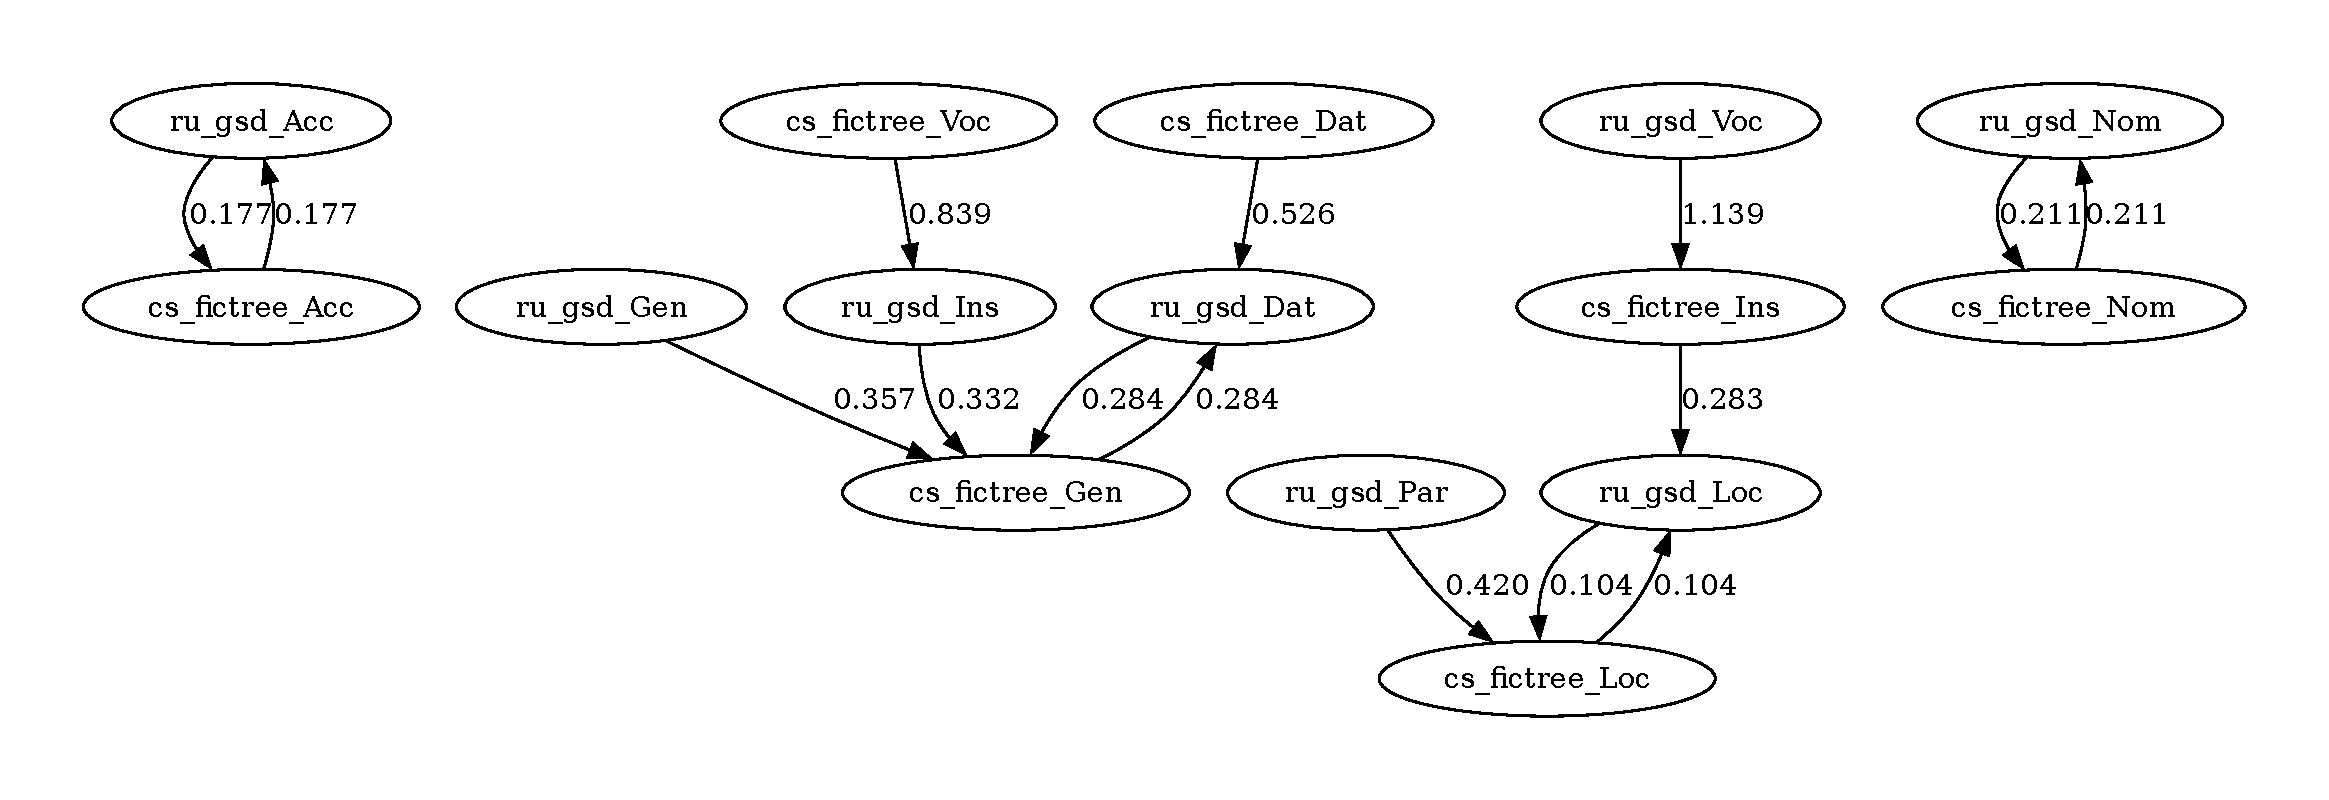
\includegraphics[width=\textwidth]{\codedir/Figures/GNN/gnn_ru_gsd_cs_fictree_Nouns_Only.pdf}
	    \caption{Graphes des Plus Proches Voisins Russe-Tchèque pour les Noms uniquement.}
    \end{figure}
    On observe notamment que pour les noms, la structure du graphe reste la même.
    Le vocatif russe et le vocatif tchèque, peu utilisées et le partitif russe n'ayant pas d'équivalent en tchèque, ils sont bien plus éloignés des autres cas.
    On retrouve par ailleurs un bloc datif -- génitif qui était déjà présent auparavant, à variance dans le corpus près.
    Par ailleurs, on observe également que les paires accusatif -- accusatif et nominatif -- nominatif restent stables et plus proches que toutes les autres paires de cas.\\
    En ne considérant que les pronoms, on obtient le graphe suivant:
    \begin{figure}[H]
	    \centering
	    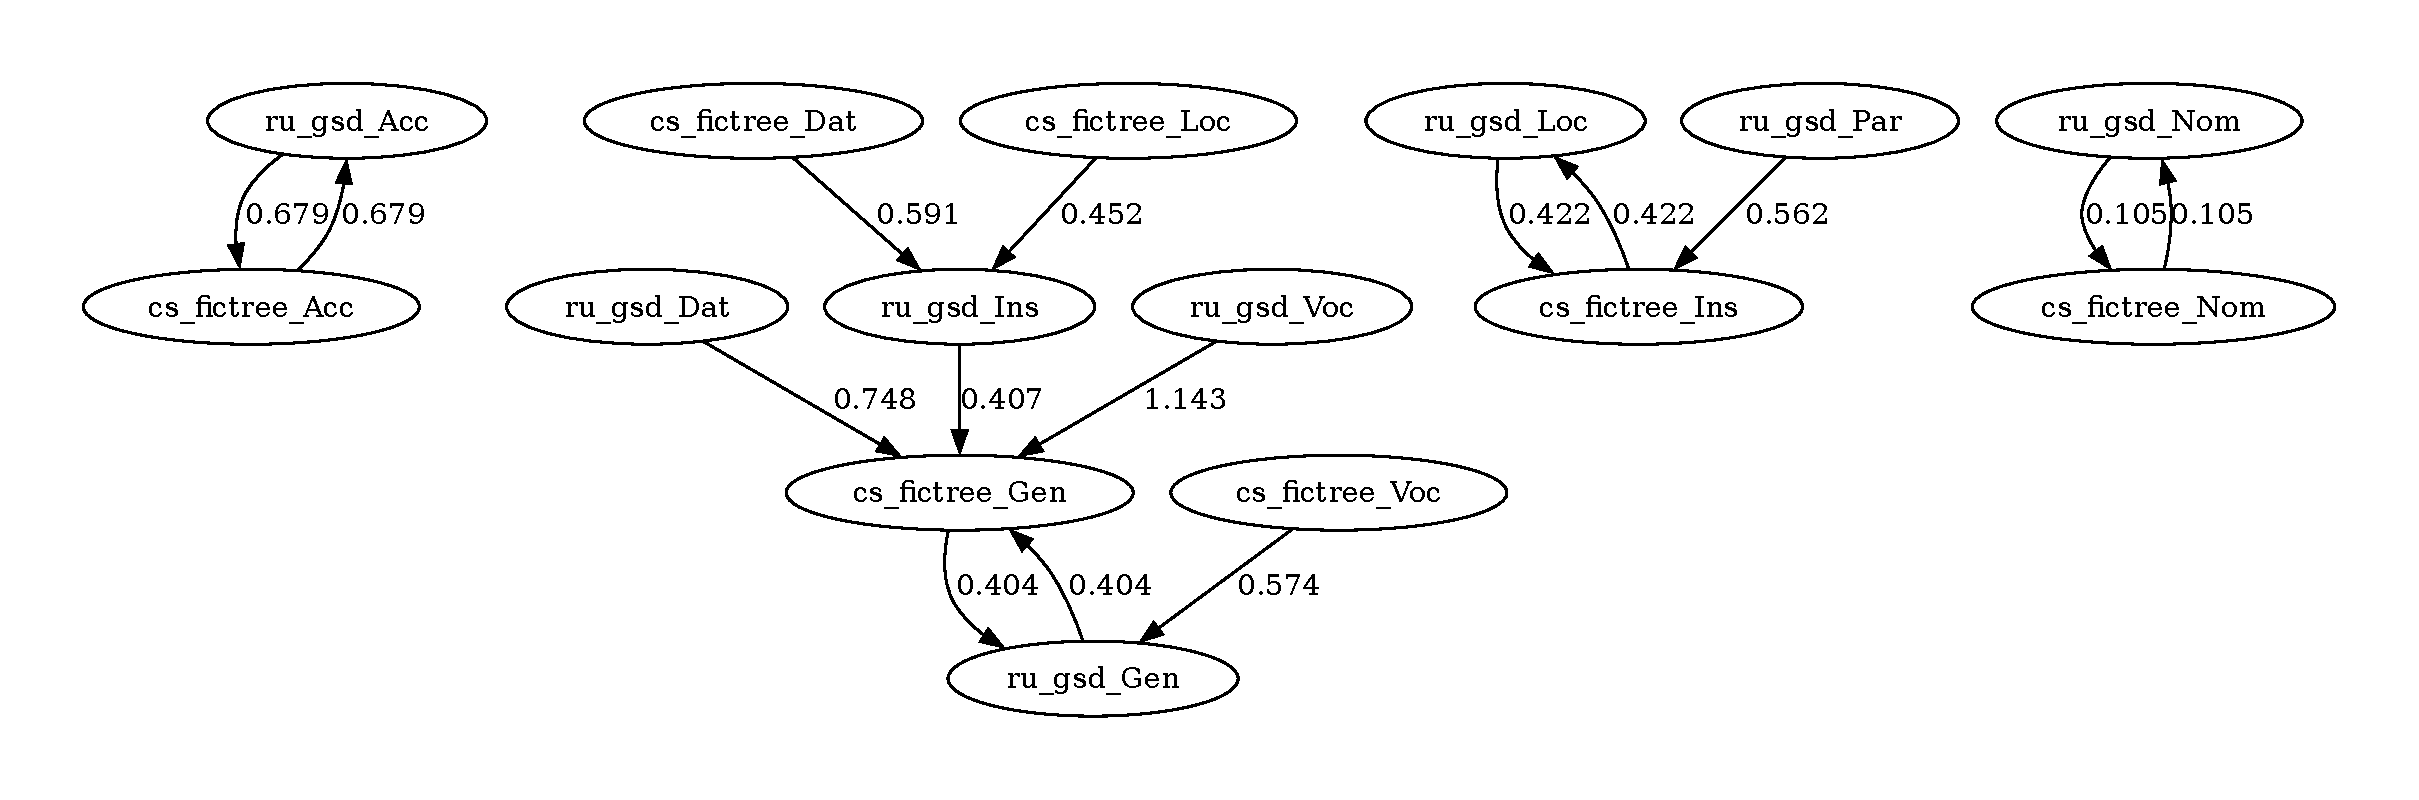
\includegraphics[width=\textwidth]{\codedir/Figures/GNN/gnn_ru_gsd_cs_fictree_Pronouns_Only.pdf}
	    \caption{Graphes des Plus Proches Voisins Russe-Tchèque pour les Pronoms uniquement.}
    \end{figure}
    Cette fois ci, il y a une variance bien plus forte dans les distances, sans doute due à la variance dans les données. En effet, à part au nominatif et à l'accusatif les échantillons de données sont bien plus faibles.
    \begin{table}[H]
	    \centering
	    \framebox{\begin{minipage}{.45\textwidth}
		    \begin{center}
			    \emph{Échantillons pour les noms:}
		    \medskip
		    \begin{tabular}{ccc}
			    \toprule
			    Cas & Russe & Tchèque\\
			    \midrule
			    Acc & 2807 & 5960\\
			    \midrule
			    Dat & 1029 & 861\\
			    \midrule
			    Gen & 7616 & 4378\\
			    \midrule
			    Ins & 1642 & 2100\\
			    \midrule
			    Loc & 2809 & 2583\\
			    \midrule
			    Nom & 4571 & 5970\\
			    \midrule
			    Par & 1 & 0\\
			    \midrule
			    Voc & 1 & 203\\
			    \bottomrule
		    \end{tabular}
	    \end{center}
	    \end{minipage}}
	    \framebox{
	    \begin{minipage}{.45\textwidth}
		    \begin{center}
			    \emph{Échantillons pour les pronoms:}
		    \medskip
	    \begin{tabular}{ccc}
		    \toprule
		    Cas & Russe & Tchèque\\
		    \midrule
		    Acc & 206 & 5960\\
		    \midrule
		    Dat & 129 & 2743\\
		    \midrule
		    Gen & 241 & 448\\
		    \midrule
		    Ins & 151 & 400\\
		    \midrule
		    Loc & 128 & 221\\
		    \midrule
		    Nom & 631 & 1427\\
		    \midrule
		    Par & 1 & 0\\
		    \midrule
		    Voc & 1 & 8\\
		    \bottomrule
	    \end{tabular}
    \end{center}
    \end{minipage}}
	    \caption{Taille d'Échantillons sur les cas en Russe et en Tchèque.}
    \end{table}
    Finalement, il semble que considérer les pronoms fait perdre en information car ceux-ci sont bien moins usités en général. Toutefois, on remarque également qu'une structure générale de la langue semble transparaitre de ces graphes.
    Il faut cependant noter que les graphes dépendent très fortement du corpus proposé:
    \begin{figure}[H]
	    \centering
	    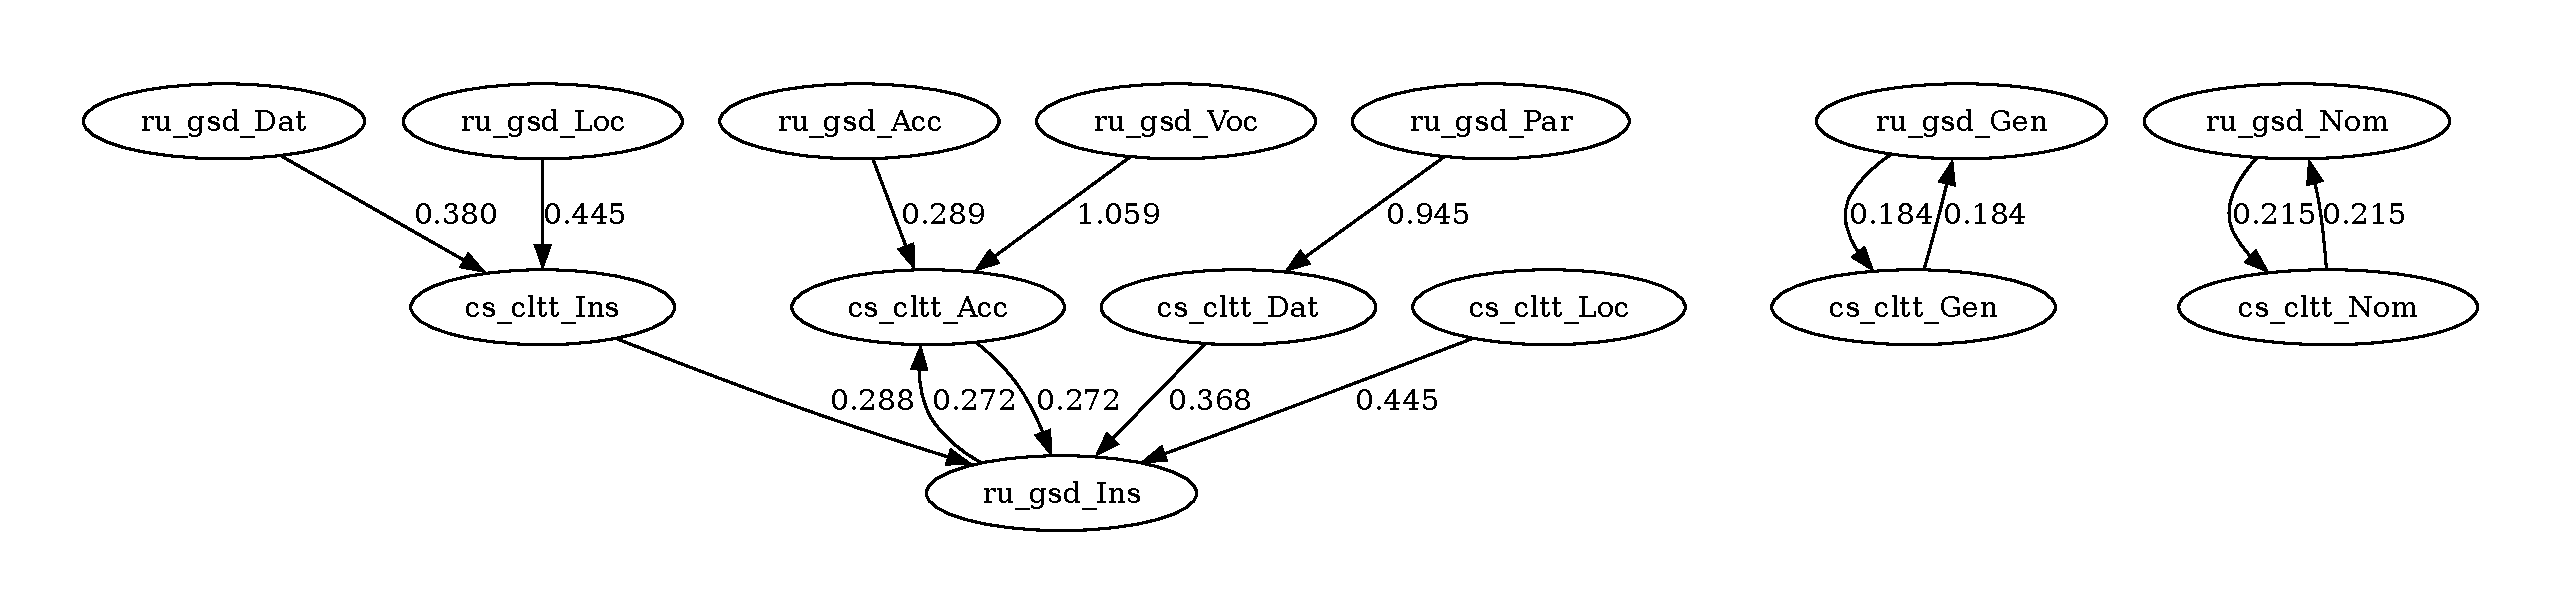
\includegraphics[width=\textwidth]{\codedir/Figures/GNN/gnn_ru_gsd_cs_cltt.pdf}
	    \caption{Graphe des Plus Proches Voisins Russe-Tchèque}
    \end{figure}
    Ici, on ne considère plus le corpus \texttt{cs\_fictree} mais le \texttt{cs\_cltt}, bien plus petit (467 phrases contre 10160).
    Même si la forme du graphe ne semble que peu changer, la variance dans le corpus joue énormément.\\
    Par ailleurs, cette méthode n'est que peu applicable, puisqu'elle nécessite d'étudier toutes les langues par paire.

\section{Visualisation des Données}
Les résultats précédemment obtenus ne permettent d'observer les données ou bien à une échelle très importante, ce qui brouille les résultats, ou bien à une échelle trop faible pour qu'on puisse généraliser un résultat.
Dans la suite, on propose donc des méthodes pour regrouper les vecteurs de cas dans différentes langues, afin d'essayer de constater l'uniformité (ou non) de certains groupes de cas.

\subsection{PCA}
On commence par appliquer une analyse en deux composantes principales (PCA) aux vecteurs représentant deux cas différents.

\begin{figure}[H]
    \begin{center}
        \begin{minipage}{.5\textwidth}
            \begin{center}
                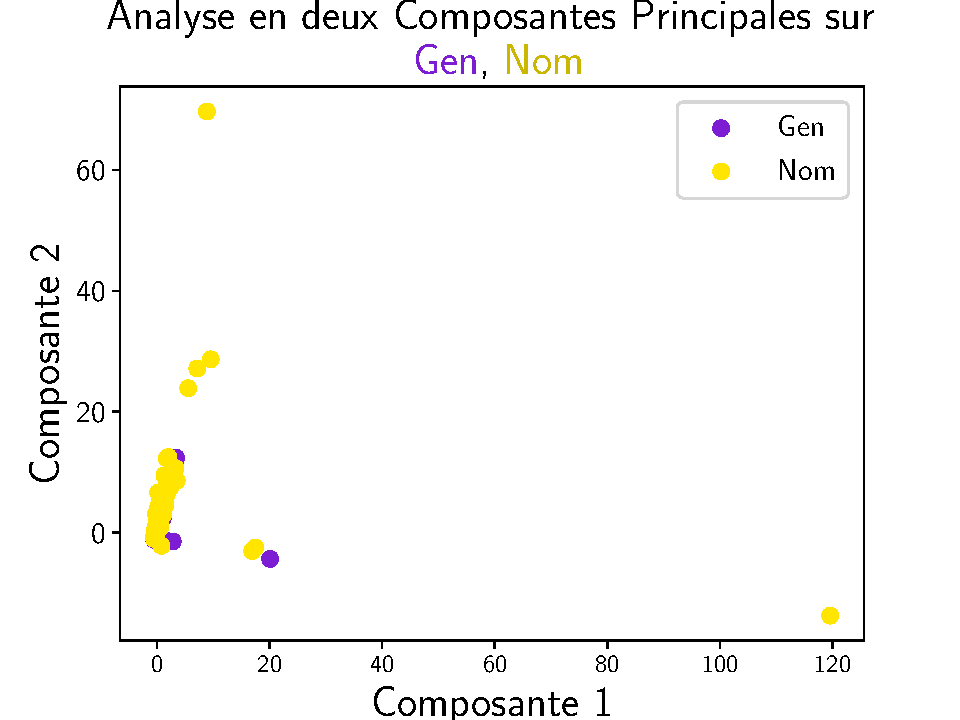
\includegraphics[width=\linewidth]{\codedir/Figures/Visualisations/pca_Gen_Nom.pdf}
            \end{center}
        \end{minipage}
    \end{center}
    \begin{minipage}{.5\textwidth}
        \begin{center}
            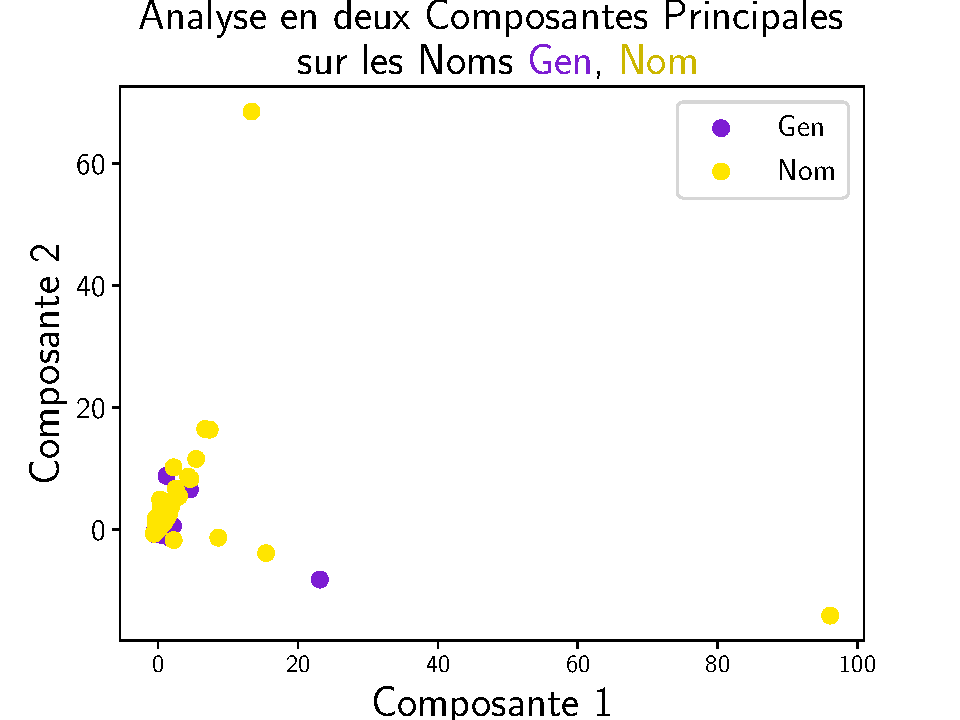
\includegraphics[width=\linewidth]{\codedir/Figures/Visualisations/pca_Gen_Nom_Nouns.pdf}
        \end{center}
    \end{minipage}
    \begin{minipage}{.5\textwidth}
        \begin{center}
            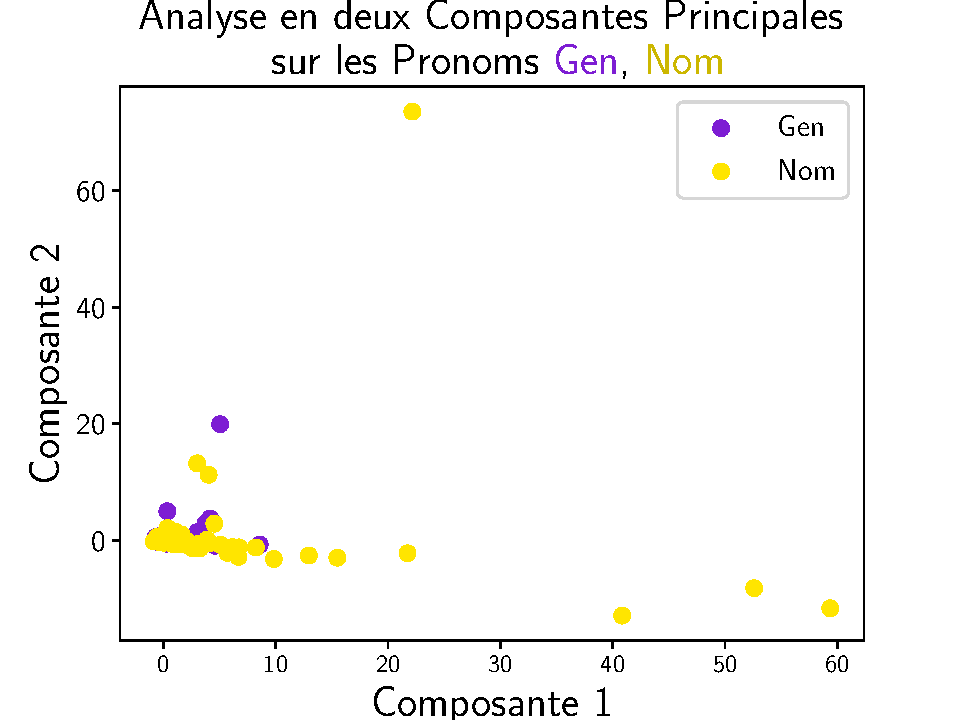
\includegraphics[width=\linewidth]{\codedir/Figures/Visualisations/pca_Gen_Nom_Pronouns.pdf}
        \end{center}
    \end{minipage}
    \caption{Représentations de l'Analyse en deux Composantes Principales sur le Génitif et le Nominatif}
\end{figure}

En regardant de plus près, les composantes déterminées par l'algorithme de PCA sont en fait des langues, et donc les deux composantes n'ont pas de sens au regard de la syntaxe.

\subsection{Clustering avec ToMATo}
L'algorithme est présenté dans \cite{ToMATo}.
\begin{figure}[H]
    \begin{center}
        \begin{minipage}{.5\textwidth}
            \begin{center}
                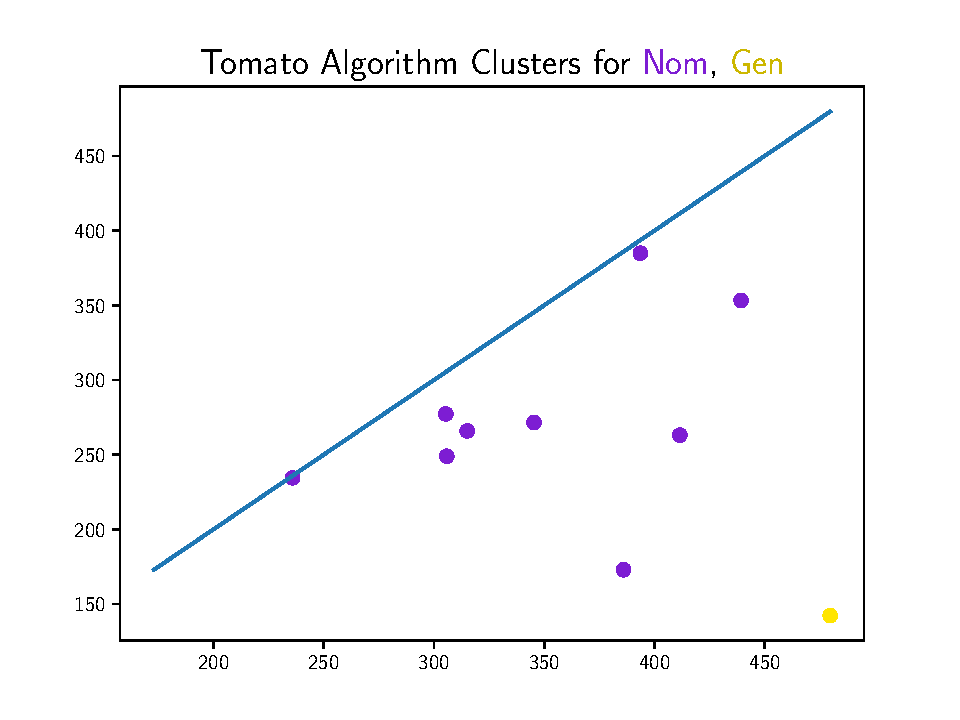
\includegraphics[width=\linewidth]{\codedir/Figures/Visualisations/tomato_Nom_Gen_Nouns.pdf}
            \end{center}
        \end{minipage}
    \end{center}

    \begin{minipage}{.5\textwidth}
        \begin{center}
            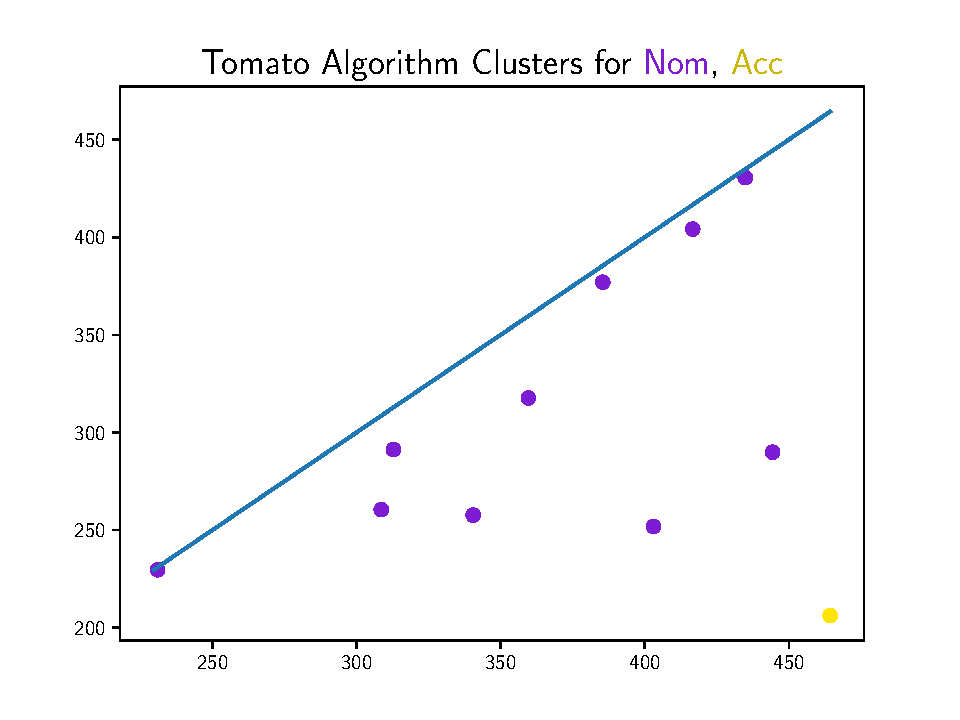
\includegraphics[width=\linewidth]{\codedir/Figures/Visualisations/tomato_Nom_Acc_Nouns.pdf}
        \end{center}
    \end{minipage}
    \begin{minipage}{.5\textwidth}
        \begin{center}
            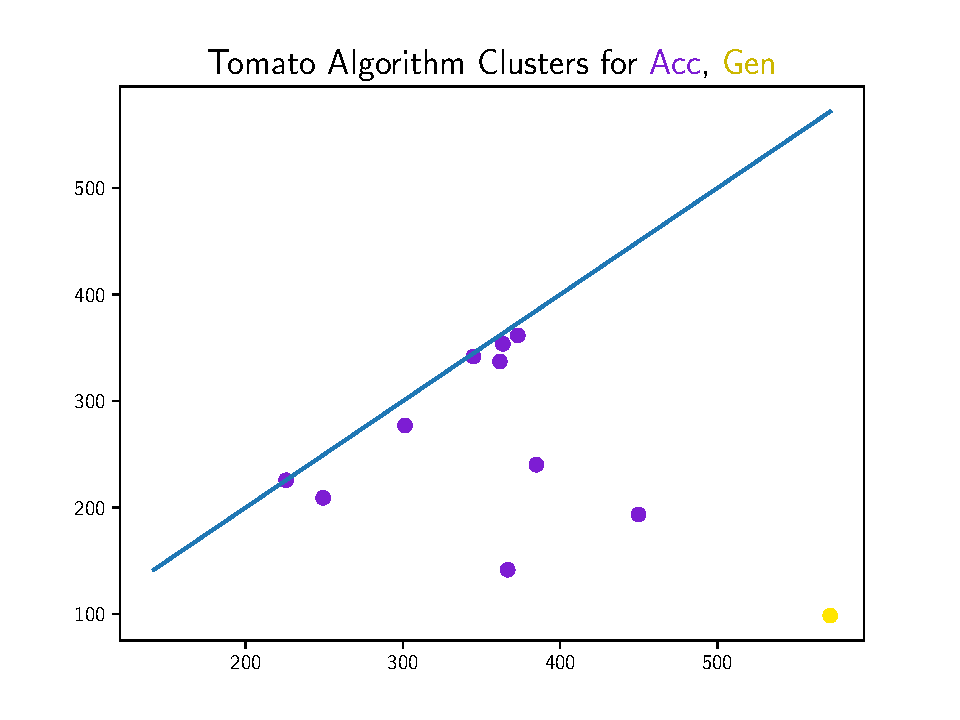
\includegraphics[width=\linewidth]{\codedir/Figures/Visualisations/tomato_Acc_Gen_Nouns.pdf}
        \end{center}
    \end{minipage}
    \caption{Représentations des clusters trouvés par l'algorithme ToMATo sur les paires de $\{\tt Acc,Nom,Gen\}$}
\end{figure}

\subsection{Analyse Topologique des Données}
Pour l'implémentation de ce qui suit, on utilise les biblothèques Python \texttt{Gudhi}, \texttt{POT} et \texttt{Hera}, dont les implémentations sont décrites dans \cite{Gudhi},\cite{PythonPOT}, \cite{Hera}
\begin{figure}[H]
    \begin{minipage}{.5\textwidth}
        \begin{center}
            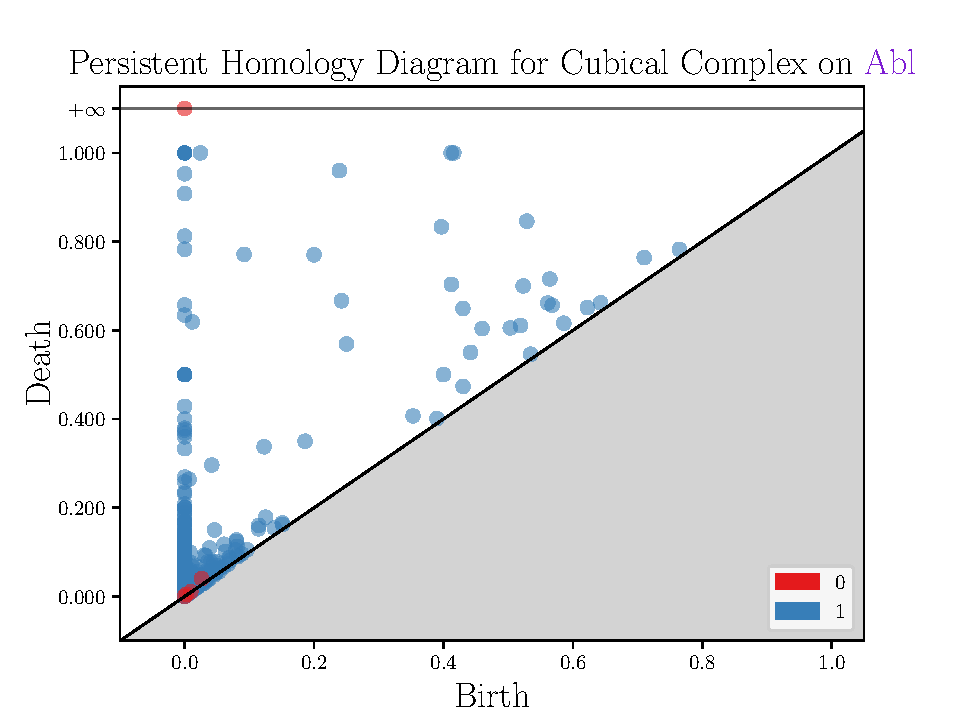
\includegraphics[width=\linewidth]{\codedir/Figures/Visualisations/cc_Abl.pdf}
        \end{center}
    \end{minipage}
    \begin{minipage}{.5\textwidth}
        \begin{center}
            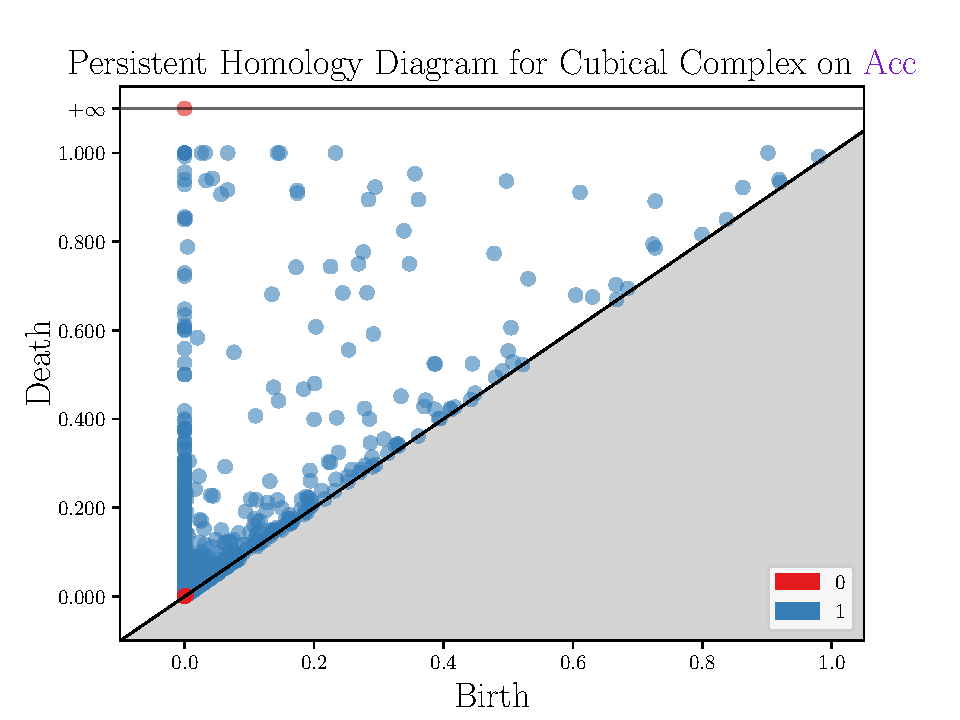
\includegraphics[width=\linewidth]{\codedir/Figures/Visualisations/cc_Acc.pdf}
        \end{center}
    \end{minipage}
    \caption{Représentations de l'Homologie Persistente du Complexe Cubique sur $\{\tt Abl,Acc\}$}
\end{figure}

\begin{figure}[H]
    \begin{minipage}{.5\textwidth}
        \begin{center}
            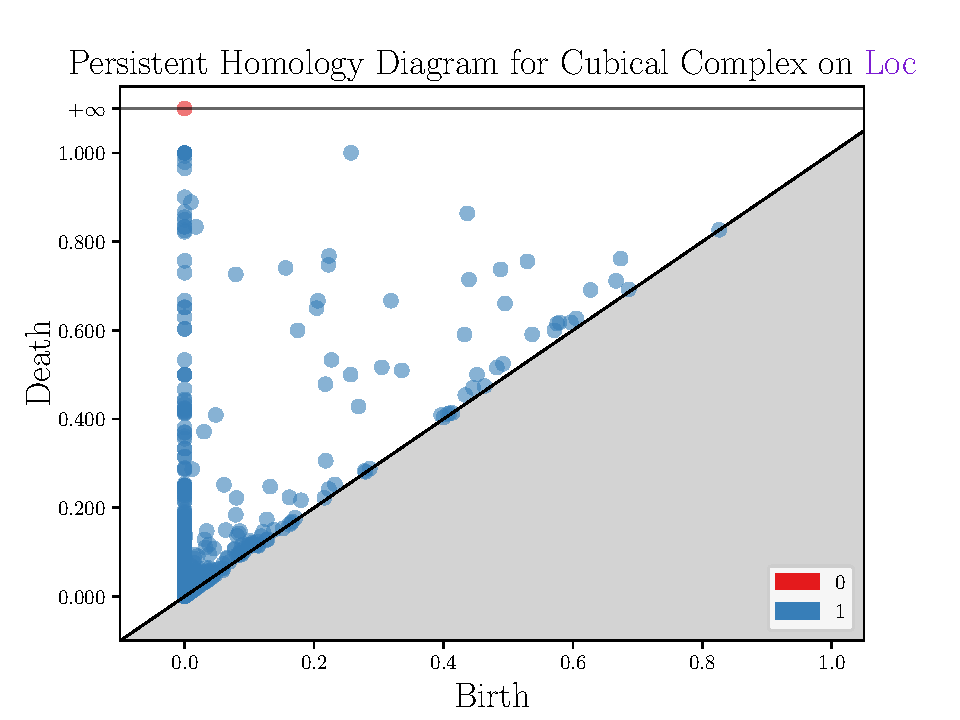
\includegraphics[width=\linewidth]{\codedir/Figures/Visualisations/cc_Loc.pdf}
        \end{center}
    \end{minipage}
    \begin{minipage}{.5\textwidth}
        \begin{center}
            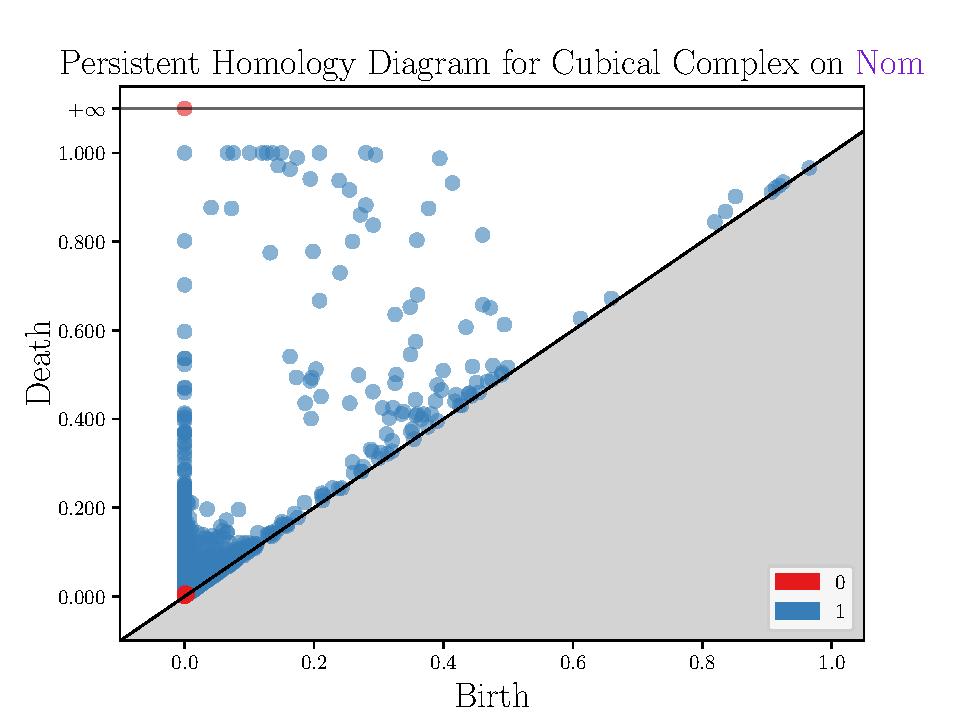
\includegraphics[width=\linewidth]{\codedir/Figures/Visualisations/cc_Nom.pdf}
        \end{center}
    \end{minipage}
    \caption{Représentations de l'Homologie Persistente du Complexe Cubique sur $\{\tt Loc,Nom\}$}
\end{figure}

On utilise un complexe cubique pour essayer de représenter au mieux les groupes d'homologie (cf.  pour les détails) de la variété triangulée par les points de chaque cas.
On remarque qu'une forme générale se retrouve dans les diagrammes de persistences de chacun des cas.
Lorsqu'on calcule la distance de Wasserstein entre deux diagrammes, on obtient le tableau suivant:
\begin{table}[H]
	\centering
	\begin{tabular}{c|ccccc}
		\toprule
		Cas & Abl & Acc & Dat & Loc & Gen\\
		\midrule
		Abl & 0.00 & 2.45 & 3.11 & 1.94 & 3.85\\
		Acc & 2.45 & 0.00 & 1.33 & 1.25 & 1.79\\
		Dat & 3.11 & 1.33 & 0.00 & 1.63 & 1.27\\
		Loc & 1.94 & 1.25 & 1.63 & 0.00 & 2.26\\
		Gen & 3.85 & 1.79 & 1.27 & 2.26 & 0.00\\
		\bottomrule
	\end{tabular}
	\caption{Distances de Wasserstein entre les Diagrammes de Persistence des Complexes Cubiques pour quelques Cas}
\end{table}
Les distances étant assez faibles, on obtient bien le résultat suggéré par les figures, il semble y avoir une structure générale de la notion topologique de variété engendrée par un cas.
Pour vérifier cette hypothèse, on teste de même en créant le complexe de Rips
Toutefois, les diagrammes restant très brouillons, il est difficile de trouver une variété plus abstraite avec la même homologie.

\begin{figure}[H]
    \begin{minipage}{.5\textwidth}
        \begin{center}
            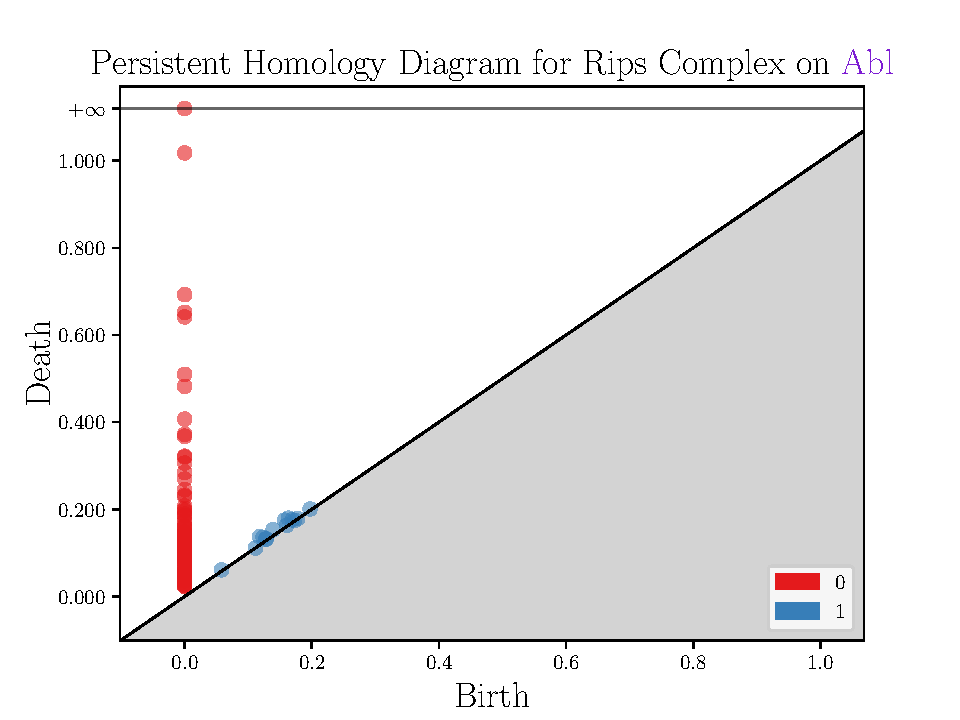
\includegraphics[width=\linewidth]{\codedir/Figures/Visualisations/rc_Abl.pdf}
        \end{center}
    \end{minipage}
    \begin{minipage}{.5\textwidth}
        \begin{center}
            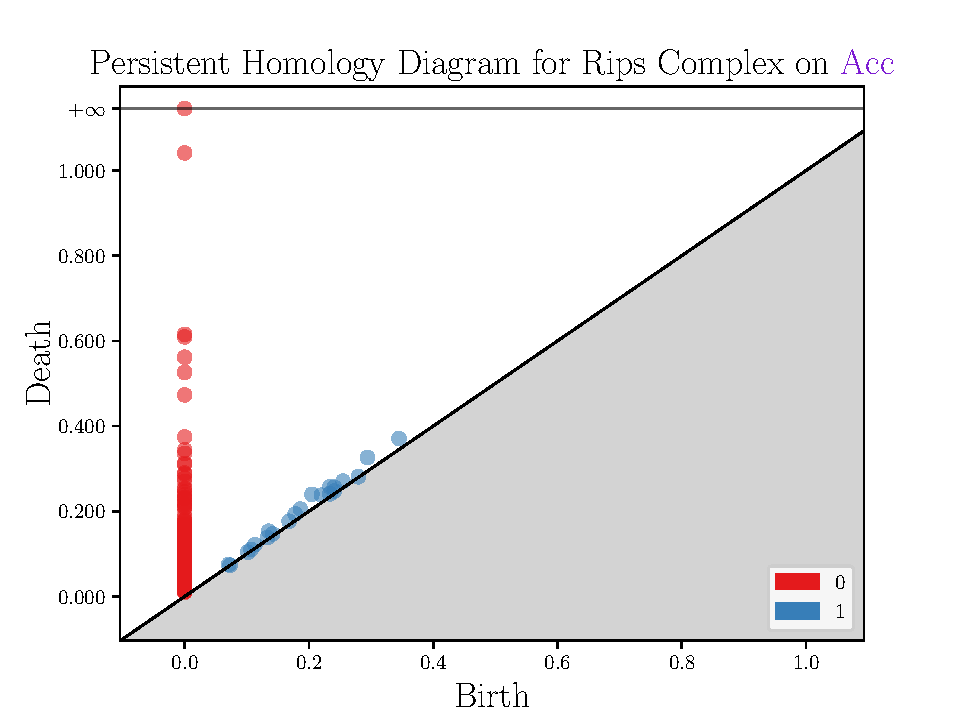
\includegraphics[width=\linewidth]{\codedir/Figures/Visualisations/rc_Acc.pdf}
        \end{center}
    \end{minipage}
    \caption{Représentations de l'Homologie Persistente du Complexe de Rips sur $\{\tt Abl,Acc\}$}
\end{figure}

\begin{figure}[H]
    \begin{minipage}{.5\textwidth}
        \begin{center}
            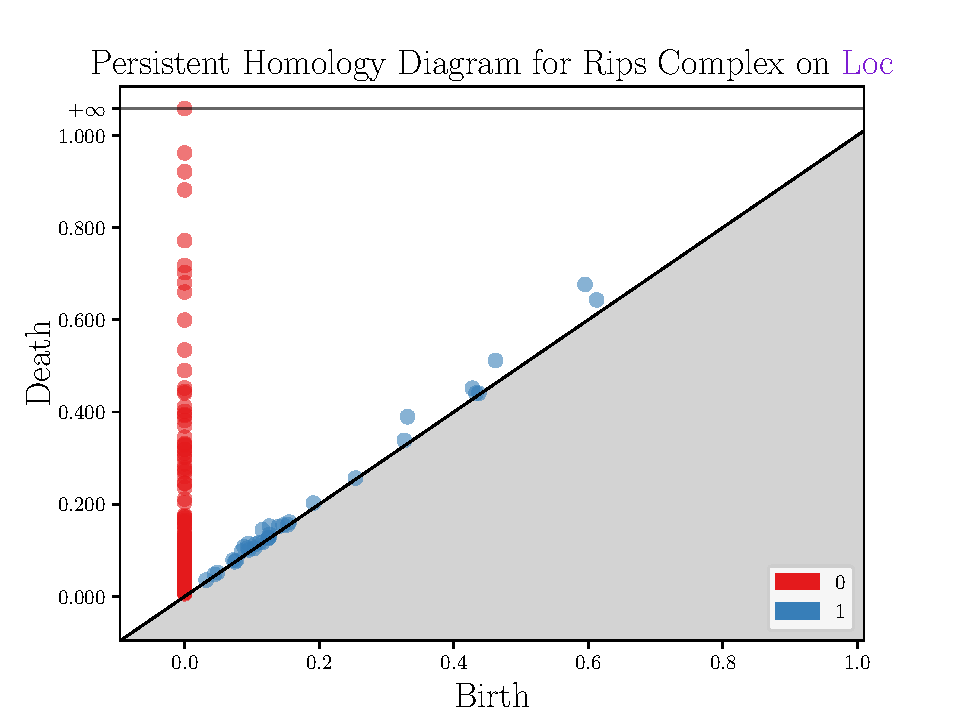
\includegraphics[width=\linewidth]{\codedir/Figures/Visualisations/rc_Loc.pdf}
        \end{center}
    \end{minipage}
    \begin{minipage}{.5\textwidth}
        \begin{center}
            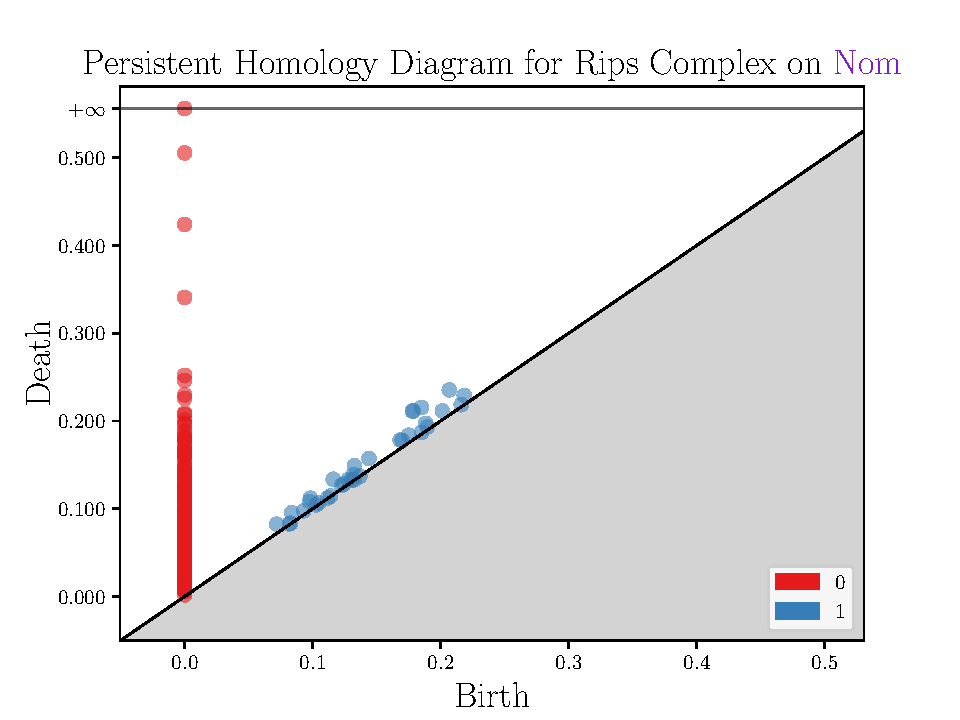
\includegraphics[width=\linewidth]{\codedir/Figures/Visualisations/rc_Nom.pdf}
        \end{center}
    \end{minipage}
    \caption{Représentations de l'Homologie Persistente du Complexe de Rips sur $\{\tt Loc,Nom\}$}
\end{figure}

On remarque à nouveau qu'une forme générale se retrouve dans les diagrammes de persistences de chacun des cas.
Lorsqu'on calcule la distance de Wasserstein entre deux diagrammes pour quelques cas, on obtient le tableau suivant:
\begin{table}[H]
	\centering
	\begin{tabular}{c|cccccc}
		\toprule
		Cas & Abl & Acc & Dat & Gen & Loc & Nom\\
		\midrule
		Abl & 0.00 & 0.89 & 1.27 & 0.82 & 1.09 & 0.94\\
		Acc & 0.89 & 0.00 & 1.01 & 0.42 & 1.03 & 0.91\\
		Dat & 1.27 & 1.01 & 0.00 & 0.87 & 1.47 & 0.76\\
		Gen & 0.82 & 0.42 & 0.87 & 0.00 & 0.84 & 0.87\\
		Loc & 1.09 & 1.03 & 1.47 & 0.84 & 0.00 & 1.48\\
		Nom & 0.94 & 0.91 & 0.76 & 0.87 & 1.48 & 0.00\\
		\bottomrule
	\end{tabular}
	\caption{Distances de Wasserstein entre les Diagrammes de Persistence des Complexes de Rips pour quelques Cas}
\end{table}


\subsection{t-SNE}
On essaie ensuite d'appliquer une analyse t-SNE en 2D, décrite dans \cite{tSNE}
\begin{figure}[H]
    \begin{center}
        \begin{minipage}{.5\textwidth}
            \begin{center}
                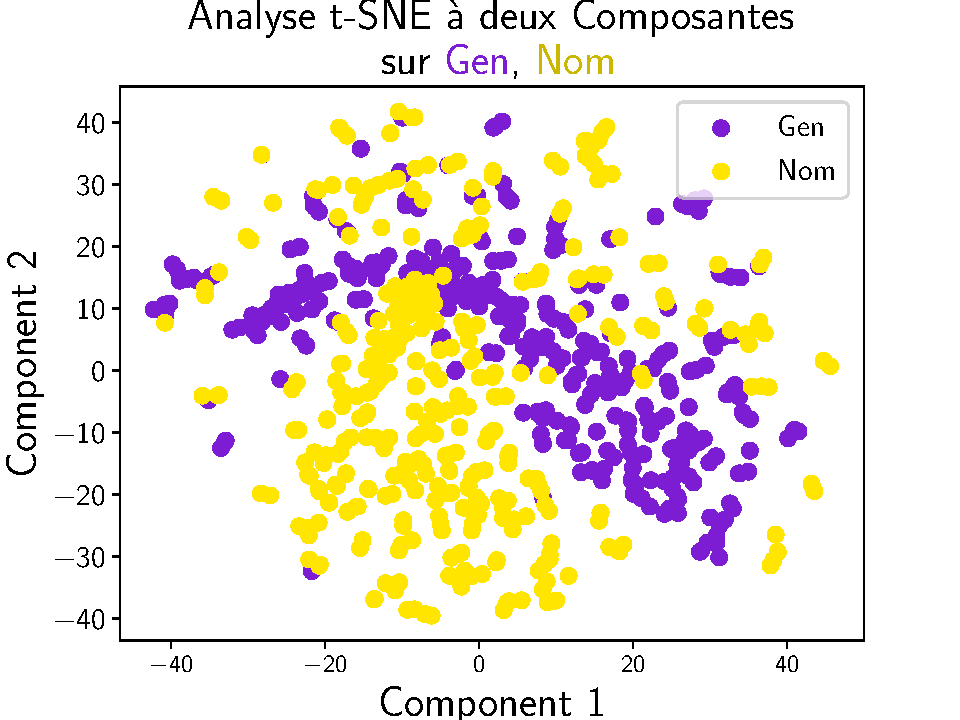
\includegraphics[width=\linewidth]{\codedir/Figures/Visualisations/tsne_Gen_Nom.pdf}
            \end{center}
        \end{minipage}
    \end{center}

    \begin{minipage}{.5\textwidth}
        \begin{center}
            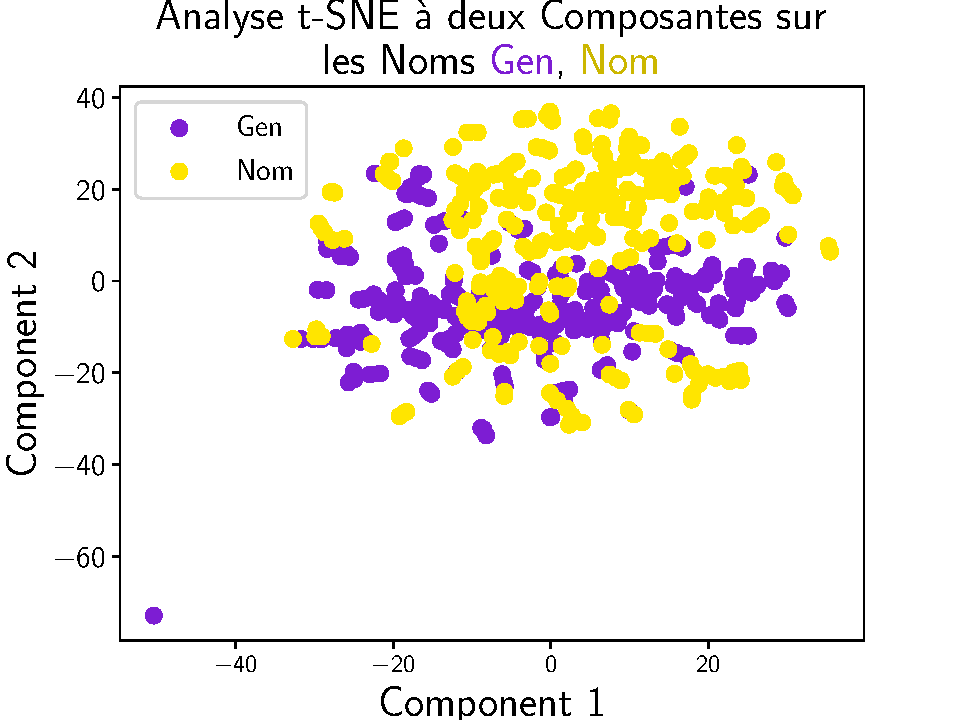
\includegraphics[width=\linewidth]{\codedir/Figures/Visualisations/tsne_Gen_Nom_Nouns.pdf}
        \end{center}
    \end{minipage}
    \begin{minipage}{.5\textwidth}
        \begin{center}
            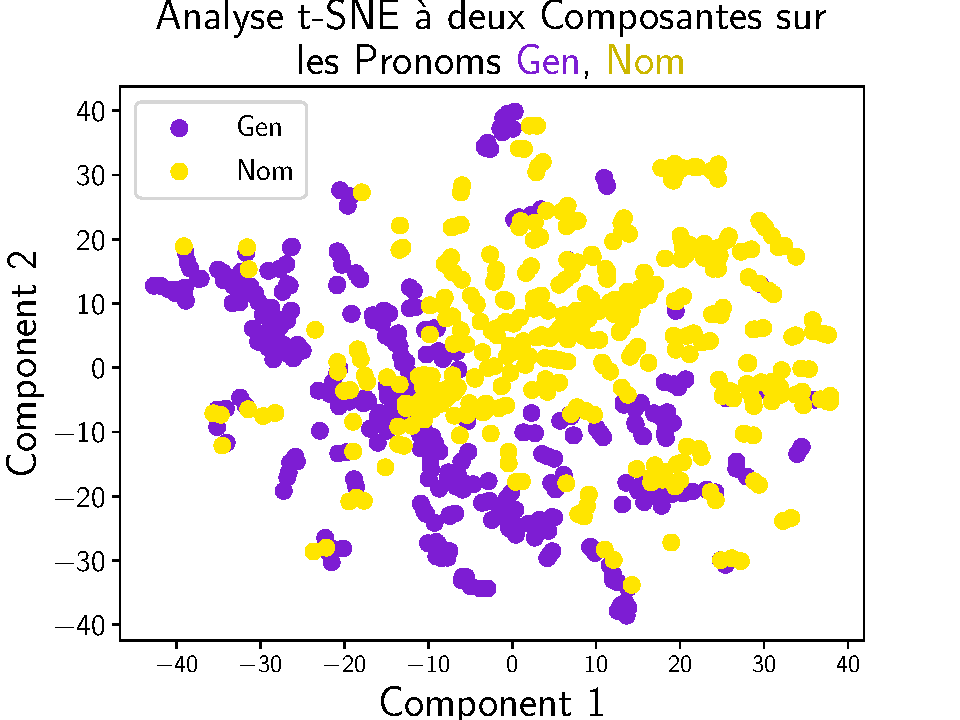
\includegraphics[width=\linewidth]{\codedir/Figures/Visualisations/tsne_Gen_Nom_Pronouns.pdf}
        \end{center}
    \end{minipage}
    \caption{Représentations de l'Analyse t-SNE à deux Composantes sur le Génitif et le Nominatif}
\end{figure}



\newpage
\appendix

\bibliography{report.bib}
\bibliographystyle{alpha-fr}

\newpage
\appendix
\tableofcontents
\listoftables
\listoffigures

\end{document}
